\documentclass{beamer}

\usepackage[utf8]{inputenc}
\usepackage[T1]{fontenc}
\usepackage{lmodern}
\usepackage{graphicx}
\usepackage{color}
%\usepackage{multirow}
\usepackage{textcomp}
\usepackage[english,french]{babel}
\usepackage{verbatim}
\usepackage{listings}


\usetheme{Luebeck}%options du thème
\usecolortheme[RGB={114,25,0}]{structure}
\setbeamertemplate{navigation symbols}{}
%\setbeamertemplate{title page}[default][colsep=-4bp,rounded=true,shadow=true]
\setbeamertemplate{blocks}[rounded][shadow=true]
\setbeamertemplate{itemize subitem}{--}
\setbeamertemplate{itemize subsubitem}{--}

\setbeamertemplate{footline}%affichage du numéro de page
{%
  \leavevmode%
  \hbox{\begin{beamercolorbox}[wd=.5\paperwidth,ht=2.5ex,dp=1.125ex,leftskip=.3cm plus1fill,rightskip=.3cm]{author in head/foot}%
    \usebeamerfont{author in head/foot}\insertshortauthor
  \end{beamercolorbox}%
  \begin{beamercolorbox}[wd=.5\paperwidth,ht=2.5ex,dp=1.125ex,leftskip=.3cm,rightskip=.3cm plus1fil]{title in head/foot}%
    \usebeamerfont{title in head/foot}\insertshorttitle \hspace{\fill}\insertframenumber{}/\inserttotalframenumber
  \end{beamercolorbox}}%
  \vskip0pt%
}

\makeatletter%commande superviser
\def\encadrant{\@dblarg\beamer@encadrant}
\long\def\beamer@encadrant[#1]#2{%
  \def\insertencadrant{\def\inst{\beamer@insttitle}\def\and{\beamer@andtitle%
  }Encadrants:\and#2}%
}
\makeatother

\setbeamertemplate{title page}%modification de la page de titre
{%
  \vbox{}
  \vfill
  \begin{centering}
%Bloc de titre
    \begin{beamercolorbox}[sep=8pt,center,colsep=-4bp,rounded=true,shadow=true]{title}
      \usebeamerfont{title}\inserttitle\par%
      \ifx\insertsubtitle\@empty%
      \else%
        \vskip0.25em%
        {\usebeamerfont{subtitle}\usebeamercolor[fg]{subtitle}\insertsubtitle\par}%
      \fi%     
    \end{beamercolorbox}%
%Auteurs
    \vskip1em\par
    \begin{beamercolorbox}[sep=8pt,center,colsep=-4bp,rounded=true,shadow=true]{author}
      \usebeamerfont{author}\insertauthor
    \end{beamercolorbox}
%Encadrants
%    \vskip0.5em\par
    \begin{beamercolorbox}[sep=8pt,center,colsep=-4bp,rounded=true,shadow=true]{encadrant}
      \footnotesize\itshape \insertencadrant
    \end{beamercolorbox}
%Etablissement
    \begin{beamercolorbox}[sep=8pt,center,colsep=-4bp,rounded=true,shadow=true]{institute}
      \usebeamerfont{institute}\insertinstitute
    \end{beamercolorbox}
%Date
    \begin{beamercolorbox}[sep=8pt,center,colsep=-4bp,rounded=true,shadow=true]{date}
      \usebeamerfont{date}\insertdate
    \end{beamercolorbox}\vskip0.5em
    {\usebeamercolor[fg]{titlegraphic}\inserttitlegraphic\par}
  \end{centering}
  \vfill
}

\newcommand{\slidepoker}[2]{
\begin{frame}[plain]
\setcounter{framenumber}{#2}
		\begin{figure}
			\includegraphics[scale=0.239]{img/s#1.jpg}
		\end{figure}
\end{frame}
}

\AtBeginSection[]%affichage du plan à chaque début de section
{
  \begin{frame}%Plan auto
    \frametitle{Plan}
    %\transdissolve
    \tableofcontents[currentsection,subsections,hideothersubsections]
  \end{frame}
}

%Profondeur de la table des matières
\setcounter{tocdepth}{1}

%\setbeameroption{show notes}
%\setbeameroption{hide notes}%default

\title{\bsc{Administration d'un serveur sous Linux}}
\subtitle{Exemple du serveur web}
\author[Averty\and Barateau\and Maloeuvre\and Percot-Tétu]{Benoit~Averty\and Yann~Barateau\and Nicolas~Maloeuvre\and Sacha~Percot-Tétu}
\institute{Institut National des Sciences Appliquées de Rennes}
\date{14 Janvier 2013}

\begin{document}

\begin{frame}
\titlepage
\end{frame}

\section*{Introduction}
%Benoit

\begin{frame}
	\frametitle{Administration système ?}
	
	\begin{itemize}
		\item Installation et mise à jour de logiciels
		\item Configuration pour une situation précise
		\item Gestion de la sécurité (contrôle d'accès, résistance aux attaques)
	\end{itemize}
    \Rightarrow Garantir les fonctionnalités du serveur et sa stabilité

    ~\\
	~\\	
	
	Pas de programmation, sauf pour automatiser des tâches

\end{frame}

\begin{frame}
	\frametitle{Objectifs du cours}
	
	\begin{itemize}
		\item Découvrir les bases de l'administration sous Linux
		\item Découvrir le fonctionnement d'un serveur web
		\item Découvrir le fonctionnement d'une application web au delà de la programmation
	\end{itemize}
\end{frame}

\begin{frame}
	\frametitle{Contexte}
	
	\begin{itemize}
		\item Distribution Debian
		\item Serveur web : Apache httpd
		\item Serveur d'applications : Apache Tomcat
	\end{itemize}
	
	~\\
	~\\	
	La plupart des notions vues s'appliquent dans d'autres cas
\end{frame}


\begin{frame}
\frametitle{Plan}
\tableofcontents
\end{frame}

\section{Généralités sur l'administration sous Linux}
%Sacha

\subsection{Objectifs du projet}
\begin{frame}{Objectifs du projet}

	Plouf
\end{frame}

\section{Apache Http Server}

\subsection{Historique}
%Yann

\begin{frame}
	\frametitle{De 1995 à aujourd'hui}
	\begin{itemize}
		\item 1995 : Version 1.0
		    \begin{itemize}
			\item collection de correctifs et d'additions au serveur NCSA HTTPd 1.3 : \og{} a patchy server \fg{}
		    \end{itemize}
        ~\\~\\
		\item 1999 : Fondation Apache
		    \begin{itemize}
		    	\item développe des logiciels open source sous la licence Apache (OpenOffice, Hadoop, Tomcat...)
		    \end{itemize}
	~\\~\\
		\item 2004 : Version 2.0
		    \begin{itemize}
		    	\item support de plusieurs plates-formes (Windows, Linux et UNIX, entre autres), support de processus légers UNIX, nouvelle API et support IPv6.
		    \end{itemize}

	\end{itemize}
\end{frame}

\begin{frame}
	\frametitle{Aujourd'hui}
	\begin{itemize}
		\item En janvier 2012, Apache Http server est toujours le serveur Web le plus populaire sur le marché.
	\end{itemize}
	\begin{center}
		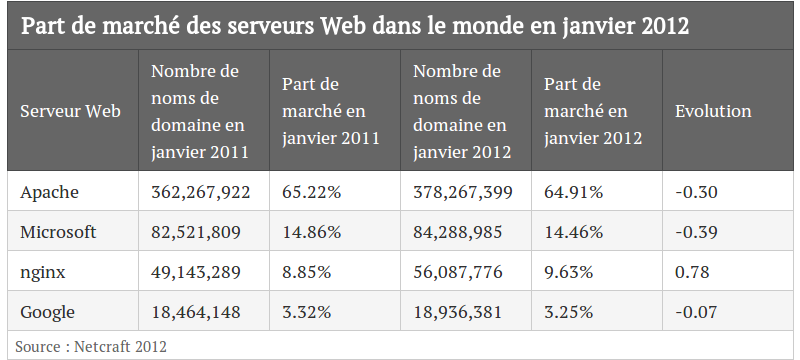
\includegraphics[scale=0.3]{Images/parts-marche.png}
	\end{center}
\end{frame}

\subsection{Fonctionnement}

\begin{frame}
	\frametitle{Fonctionnement (1/3)}
	\begin{itemize}
		\item On appelle \og{} serveur Web \fg{} à la fois le matériel informatique et le serveur Http.
	\end{itemize}
	\begin{center}
		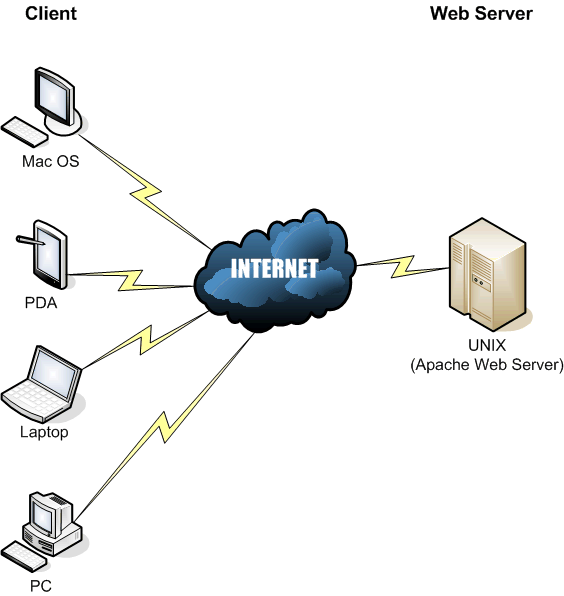
\includegraphics[scale=0.25]{Images/nuage-apache.png}
	\end{center}
\end{frame}

\begin{frame}
	\frametitle{Fonctionnement (2/3)}
	\begin{itemize}
		\item Le serveur Http attend des requêtes Http et répond en envoyant au client la page web désirée.
	\end{itemize}
	\begin{center}
		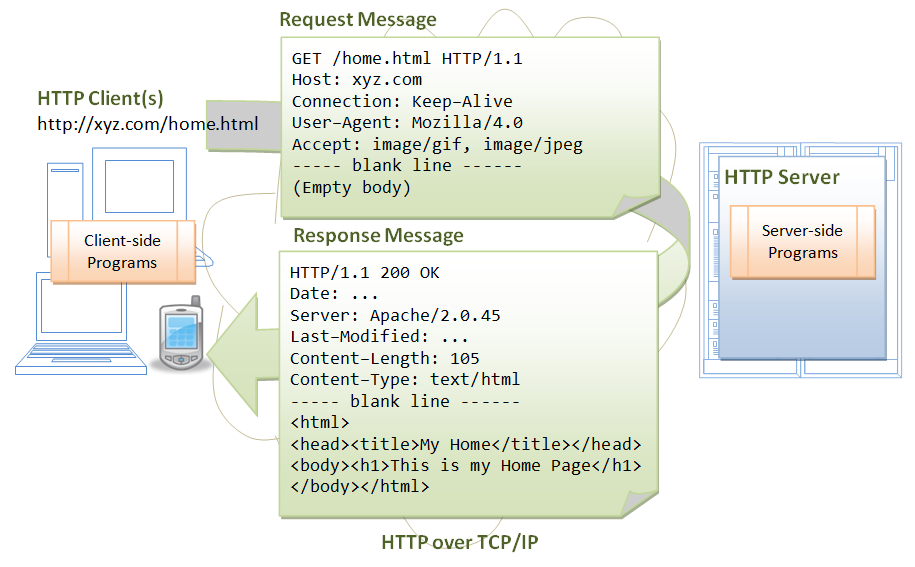
\includegraphics[scale=0.3]{Images/protocole_http.png}
	\end{center}
\end{frame}

\begin{frame}
	\frametitle{Fonctionnement (3/3)}
	\begin{itemize}
		\item Le traitement des requêtes Http par le serveur Apache se fait en plusieurs étapes.
	\end{itemize}
	\begin{center}
		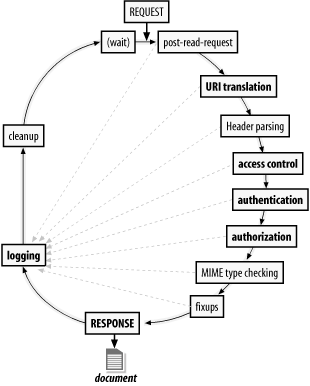
\includegraphics[scale=0.4]{Images/processing_apache.png}
	\end{center}
\end{frame}

\subsection{Fichiers de configuration}

\begin{frame}
	\frametitle{Fichiers de configuration (1/3)}
	\begin{itemize}
		\item Les fichiers de configuration se trouvent dans /etc/apache2
	\end{itemize}
	\begin{center}
		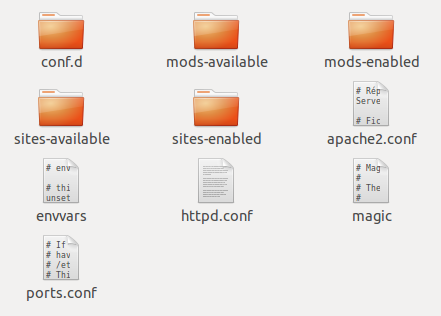
\includegraphics[scale=0.3]{Images/fichiers_config.png}
	\end{center}
\end{frame}

\begin{frame}
	\frametitle{Fichiers de configuration (2/3)}
	\begin{itemize}
	      \item Apache2.conf
	      \begin{itemize}
		  \item Ce fichier est le fichier de configuration de base. Il inclut tous les autres fichiers de configuration.
	      \end{itemize}
	      \item Ports.conf
	      \begin{itemize}
		  \item Il contient la spécification des interfaces sur lesquelles Apache écoutera les requêtes.
	      \end{itemize}
	\end{itemize}
	\begin{center}
		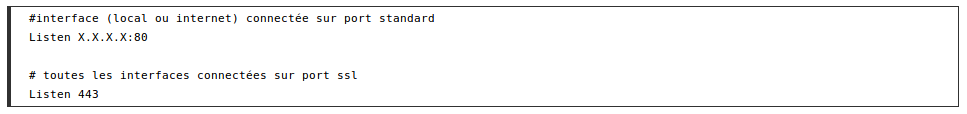
\includegraphics[scale=0.3]{Images/ports.png}
	\end{center}
\end{frame}

\begin{frame}
	\frametitle{Fichiers de configuration (3/3)}
	\begin{itemize}
	      \item Sites-available
	      \begin{itemize}
		  \item Ce dossier contient différents \textit{virtual hosts}. Il permet de définir plusieurs sites sur une même machine. Par exemple, on peut définir des sous-domaines (ex : machin.domain.tld), ainsi que d'autres domaines (ex : autredomain.tld). Les sites activés sont placés dans le dossier sites-enabled.
	      \end{itemize}
	\end{itemize}
	\begin{center}
		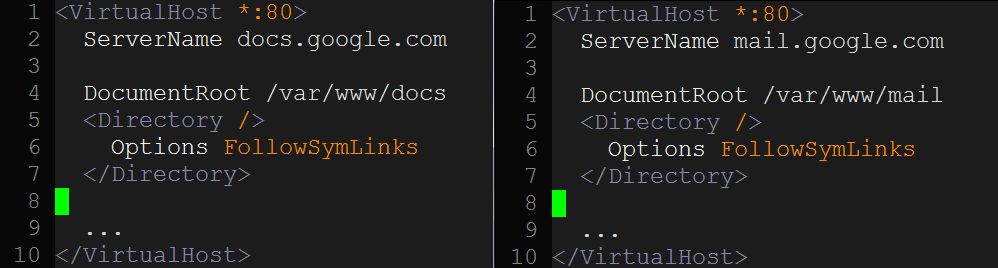
\includegraphics[scale=0.4]{Images/sites-available.png}
	\end{center}
\end{frame}

\subsection{Les modules}

\begin{frame}
	\frametitle{Les modules}
	\begin{itemize}
	  \item Il est possible d'ajouter des modules à apache, ajoutant ainsi des fonctionnalités au serveur web. Ces modules sont dans le dossier \textit{mods-available}.
	  \item On exécute le fichier .load correspondant à un module pour charger celui-ci. Le module apparaît alors dans le dossier \textit{mods-enabled}.
	  \item Lors du TP, nous utiliserons le module \textit{mod\_actions}. Celui-ci possède une directive \textit{Action} qui permet d'exécuter des scripts CGI lorsqu'un certain type de contenu MIME est requis.
	\end{itemize}
\end{frame}


\section{Tomcat : conteneur de servlet Java EE}
%Nicolas
\subsection{Presentation}
\begin{frame}
  \frametitle{Présentation de Tomcat}

  \begin{itemize}
    \item Projet open-source de la fondation Apache
    \item Serveur d'applications Java
    \begin{itemize}
      \item Servlet (génération de page Html, xml etc...)
      \item JavaServer Pages
    \end{itemize}
    \item spécifications du Java Community Process
  \end{itemize}
  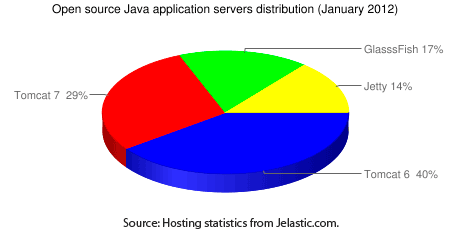
\includegraphics[scale=0.5]{Images/marcheJEE.png}
\end{frame}

\begin{frame}
  \frametitle{Autres serveurs d'applications existants}
En réalité, Tomcat est seulement un conteneur de servlets, il existe des serveurs implémentant les normes JEE (sécurité, EJB, transactions globales...) :
\begin{itemize} 
  \item GlassFish (Développé par Oracle)
  \item jBoss (Utilise Tomcat pour la partie Servlet/JSP)
  \item Websphere (IBM)
  \item ...
\end{itemize}
\end{frame}

\begin{frame}
  \frametitle{Présentation Tomcat}
  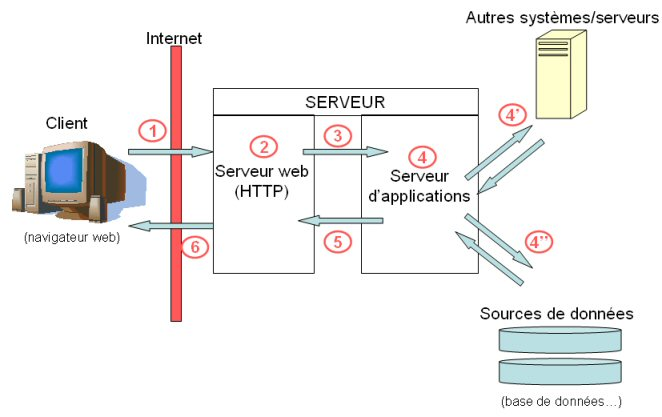
\includegraphics[scale=0.5]{Images/serveurapp.png}
\end{frame}

\subsection{Configuration}
\begin{frame}
  \frametitle{Fichiers de configuration}

		Répertoire d'installation : CATALINA\_HOME
\begin{itemize} 
    \item \textbf{bin/} exécutables de Tomcat(démarrage du serveur)
    \item \textbf{common/} classes et librairies partagées par les applications web
    \item \textbf{conf/} Fichiers de configuration
    \item \textbf{Logs/} Logs d'accès, erreurs...
    \item \textbf{server/} contient les applications web du serveur en lui-même
    \item \textbf{shared/} contient les classes et librairies partagées par toutes les applications web hébergées sur le serveur
    \item \textbf{temp/}
    \item \textbf{webapps/} contient les applications web
    \item \textbf{work/} contient les JSP compilées
\end{itemize} 
\end{frame}


\begin{frame}[fragile]
  \frametitle{conf/server.xml}

\begin{itemize}
  \item \$CATALINA\_HOME/server.xml : principal fichier de configuration
  \item Eléments conteneurs (obligatoires) : Engine, Host, Connector
  \item Définition des services, protocoles, port utilisés, redirection vers des ressources externes, des serveurs externes
  \item Eléments facultatifs : GlobalNamingResources, Resources, Realm et Valve.
\end{itemize} 

\begin{lstlisting}
  <Server port="8009" shutdown="SHUTDOWN">
  ...
  </Server>
\end{lstlisting}
		
\end{frame}


\begin{frame}[fragile]
  \frametitle{conf/server.xml}
		Elément Connecteur
		\begin{itemize} 
   		\item objet Java capable d'écouter un port précis et comprenant un protocole précis
    	\item redirige les requêtes qu'il reçoit au moteur de servlets
      \item C'est l'élément qui reçoit les requêtes HTTP et les transmet au conteneur de servlet
		\end{itemize}

        \begin{lstlisting}
<Connector port="8080"
    protocol="HTTP/1.1"
    connectionTimeout="20000"
    maxThread="100"
    maxCount="100"
    redirectPort="8443" />
        \end{lstlisting}
\end{frame}

\begin{frame}[fragile]
    \frametitle{conf/server.xml}
		Eléments Engine et Host
		\begin{itemize}
   		\item \textbf{Elément Engine} : modélise le moteur de servlet, contient un ou plusieurs hosts
    	\item \textbf{Elément Host} hôte virtuel (Similaire aux virtualhosts d'Apache)
		\end{itemize}

        \begin{lstlisting}
<Engine name="Catalina">
  <Host name="localhost" appBase="webapps"
    unpackWARs="true" autoDeploy="true">
    <!-- contenu de l'element Host -->
  </Host>
</Engine>
        \end{lstlisting}
\end{frame}

\begin{frame}[fragile]
  \frametitle{conf/server.xml}
		Resssources et variables d'environnement

        \begin{lstlisting}
<GlobalNamingResources>
  <Resource name="UserDatabase" auth="Container" type="org.apache.catalina.UserDatabase" description="User database that can be updated and saved" factory="org.apache.catalina.users.MemoryUserDatabaseFactory" pathname="conf/tomcat-users.xml" />
  <Environment name="maxRetry" type="java.lang.Integer" value="10" override="false"/>
</GlobalNamingResources>

        \end{lstlisting}
\end{frame}

\subsection{Déploiement d'une application}
\begin{frame}
\frametitle{Via le manager}
	Installation d'une application web sous la forme d'une archive war
  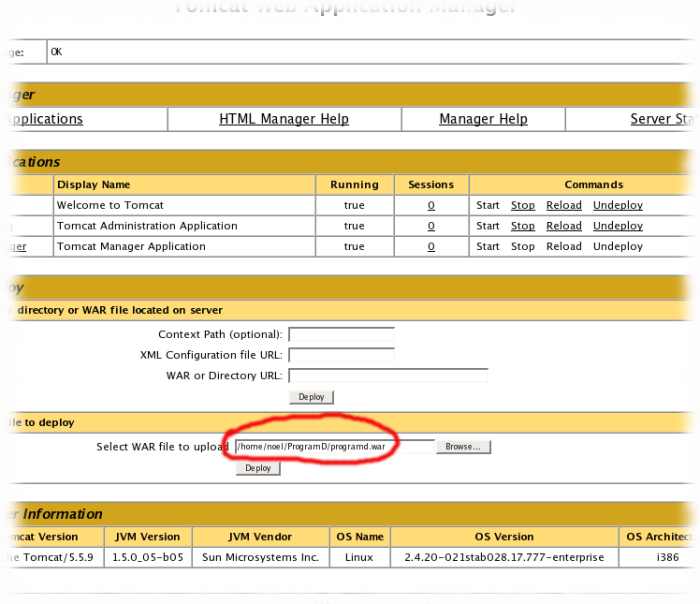
\includegraphics[scale=0.3]{Images/tomcat-deploy-war.png}
\end{frame}

\begin{frame}
  \frametitle{Directement dans le dossier de Tomcat}

  \begin{itemize}
    \item Placer l'archive war dans le dossier webapps/
    \item Tomcat décompresse l'application au démarrage
    \item L'application est accessible par l'url http://serveur.tld/nom\_archive\_war
  \end{itemize}
\end{frame}


\section{mod\_jk : Relier Apache et Tomcat}
%Benoit

\subsection{Avantages}
\begin{frame}
	\begin{itemize}
		\item Apache + Tomcat sur la même machine et sur le même port
		\item Ressources statiques servies par Apache (meilleures performances)
		\item Utilisation de la configuration avancée d'Apache sur une application Java (url rewriting, htaccess...)
		\item Load balancing via le mod jk.
	\end{itemize}
\end{frame}

\subsection{Utilisation des mods}
\begin{frame}
	\frametitle{Fichiers importants}
	
	\begin{itemize}
		\item \textbf{/usr/lib/apache2/modules/mod\_x.so} :\\~~~~ Le code du module
		\item \textbf{/etc/apache2/mods-available/x.load} :\\~~~~ Instructions de chargement du module (LoadModule)
		\item \textbf{/etc/apache2/mods-available/x.conf} :\\~~~~ Configurations du module
	\end{itemize}
	
\end{frame}

\begin{frame}
	\frametitle{Utilisation d'un module}

	Fonctionnement similaire aux virtualhosts
	
	\begin{itemize}
		\item Apache lis les fichiers présents dans /etc/apache2/mods-enabled
		\item Activation d'un module : lien symbolique vers mods-available/x.load dans mods-enabled/
		\item Tâche facilitée par la commande a2enmod (apache2 enable mod)	
	\end{itemize}
	
\end{frame}

\subsection{Configuration de mod\_jk}
\begin{frame}
	\frametitle{Fonctionnement}
	
	\begin{itemize}
		\item Configuration de \og{} workers \fg{} (workers.properties)
		\item Inclusion de la configuration dans Apache (option JkWorkersFile)
		\item Redirection de certaines requêtes vers un worker (option JkMount)
	\end{itemize}
\end{frame}

\begin{frame}
	\frametitle{Fichier workers.properties}
	
	\begin{itemize}
		\item Présent dans /etc/libapache2-mod-jk/		
		\item Inclus via l'option JkWorkersFile dans mods-available/jk.conf
	\end{itemize}

	
	\begin{center}
		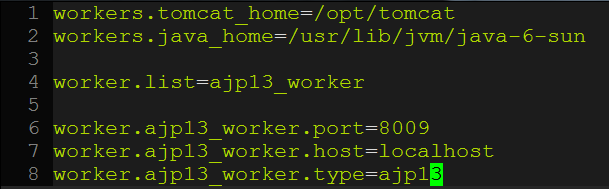
\includegraphics[scale=0.6]{Images/workers-properties.png}
	\end{center}
\end{frame}

\begin{frame}
	\frametitle{Redirection des requêtes}
	
	\begin{itemize}
		\item Option JkMount <url> <worker\_name>		
		\item En général spécifique à un virtualhost
	\end{itemize}

	\begin{center}
		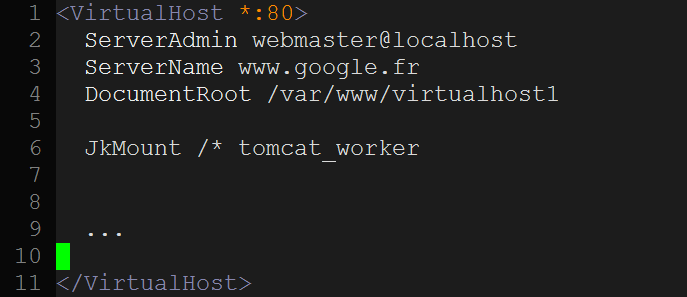
\includegraphics[scale=0.5]{Images/jkmount-example.png}
	\end{center}

\end{frame}


\end{document}

